\documentclass[11pt,a4paper]{article}
\usepackage[utf8]{inputenc}
\usepackage[english]{babel}
\usepackage[left=2.5cm, right=2.5cm, top=2.5cm, bottom=2.5cm]{geometry}
\usepackage{hyperref}
\usepackage{graphicx}
\usepackage{times}
\usepackage[bottom]{footmisc}
\usepackage{listings}
\usepackage{bm}
\usepackage{amsmath}
\usepackage{algpseudocode}
\usepackage{algorithm}
\usepackage{titlesec}
\usepackage{booktabs}
\usepackage{amsmath}
\usepackage{xfrac}


\title{\textbf{Advanced Machine Learning -- Homework 2}}
\author{Anna Berger, Ashwin Sadananda Bhat (AML25)}


\begin{document}
	\maketitle
	
	\section*{Part 1: Mixture Models}
	\subsection*{Exercise 1.1}
	
	In this part we consider the mixture of two Bernoulli distributions. To be more specific: each observation $x=(h, t)$ is the outcome of 5 coin tosses with a specific coin, with $h$ --- the number of heads and $t$ --- the number of tails, so $h+t=5$. But there are two coins in play with possible different probabilities for heads. Hence it can be modelled as a mixture of two probability distributions:
	$$ p(x | \mu,\pi) = \pi_1 \cdot p(x|\mu_1) + \pi_2 \cdot p(x|\mu_2) $$
	
	Each probability distribution is of Bernoulli type, so:
	$$ p((h,t)|\mu) = \binom {h+t}{h} \cdot \mu^h \cdot (1-\mu)^t$$
	
	We assume that parameters of the model are initialised as $\pi = \left(
	 \frac{1}{3}, \frac{2}{3}\right)$, $\mu = \left(
	 \frac{2}{3}, \frac{1}{2}\right)$.
	
	First, for each observation and for each component we compute responsibilities:
	
	$$ \gamma(z_{11}) = \frac{\pi_1 \cdot p(x_1|\mu_1)}{\pi_1 \cdot p(x_1|\mu_1)+[\pi_2 \cdot p(x_1|\mu_2)} = \frac{\binom {5}{2} \cdot \frac{1}{3} \cdot (\frac{2}{3})^2 \cdot (\frac{1}{3})^3}{\binom {5}{2} \cdot \frac{1}{3} \cdot (\frac{2}{3})^2 \cdot (\frac{1}{3})^3+\binom {5}{2} \cdot \frac{2}{3} \cdot (\frac{1}{2})^2 \cdot (\frac{1}{2})^3}=\frac{64}{307} $$
	
	$$ \gamma(z_{12}) = \frac{\pi_2 \cdot p(x_1|\mu_2)}{\pi_1 \cdot p(x_1|\mu_1)+\pi_2 \cdot p(x_1|\mu_2)} = \frac{\binom {5}{2} \cdot \frac{2}{3} \cdot (\frac{1}{2})^2 \cdot (\frac{1}{2})^3}{\binom {5}{2} \cdot \frac{1}{3} \cdot (\frac{2}{3})^2 \cdot (\frac{1}{3})^3+\binom {5}{2} \cdot \frac{2}{3} \cdot (\frac{1}{2})^2 \cdot (\frac{1}{2})^3}=\frac{243}{307} $$
	
	$$ \gamma(z_{21}) = \frac{\pi_1 \cdot p(x_2|\mu_1)}{\pi_1 \cdot p(x_2|\mu_1)+\pi_2 \cdot p(x_2|\mu_2)} = \frac{\binom {5}{1} \cdot \frac{1}{3} \cdot (\frac{2}{3})^1 \cdot (\frac{1}{3})^4}{\binom {5}{1} \cdot \frac{1}{3} \cdot (\frac{2}{3})^1 \cdot (\frac{1}{3})^4+\binom {5}{1} \cdot \frac{2}{3} \cdot (\frac{1}{2})^1 \cdot (\frac{1}{2})^4}=\frac{32}{275} $$
	
	$$ \gamma(z_{22}) = \frac{\pi_2 \cdot p(x_2|\mu_2)}{\pi_1 \cdot p(x_2|\mu_1)+\pi_2 \cdot p(x_2|\mu_2)} = \frac{\binom {5}{1} \cdot \frac{2}{3} \cdot (\frac{1}{2})^1 \cdot (\frac{1}{2})^4}{\binom {5}{1} \cdot \frac{1}{3} \cdot (\frac{2}{3})^1 \cdot (\frac{1}{3})^4+\binom {5}{1} \cdot \frac{2}{3} \cdot (\frac{1}{2})^1 \cdot (\frac{1}{2})^4}=\frac{243}{275} $$
	
	$$ \gamma(z_{31}) = \frac{\pi_1 \cdot p(x_3|\mu_1)}{\pi_1 \cdot p(x_3|\mu_1)+\pi_2 \cdot p(x_3|\mu_2)} = \frac{\binom {5}{2} \cdot \frac{1}{3} \cdot (\frac{2}{3})^2 \cdot (\frac{1}{3})^3}{\binom {5}{2} \cdot \frac{1}{3} \cdot (\frac{2}{3})^2 \cdot (\frac{1}{3})^3+\binom {5}{2} \cdot \frac{2}{3} \cdot (\frac{1}{2})^2 \cdot (\frac{1}{2})^3}=\frac{64}{307} $$
	
	$$ \gamma(z_{32}) = \frac{\pi_2 \cdot p(x_3|\mu_2)}{\pi_1 \cdot p(x_3|\mu_1)+\pi_2 \cdot p(x_3|\mu_2)} = \frac{\binom {5}{2} \cdot \frac{2}{3} \cdot (\frac{1}{2})^2 \cdot (\frac{1}{2})^3}{\binom {5}{2} \cdot \frac{1}{3} \cdot (\frac{2}{3})^2 \cdot (\frac{1}{3})^3+\binom {5}{2} \cdot \frac{2}{3} \cdot (\frac{1}{2})^2 \cdot (\frac{1}{2})^3}=\frac{243}{307} $$
	
	$$ \gamma(z_{41}) = \frac{\pi_1 \cdot p(x_4|\mu_1)}{\pi_1 \cdot p(x_4|\mu_1)+\pi_2 \cdot p(x_4|\mu_2)} = \frac{\binom {5}{3} \cdot \frac{1}{3} \cdot (\frac{2}{3})^3 \cdot (\frac{1}{3})^2}{\binom {5}{3} \cdot \frac{1}{3} \cdot (\frac{2}{3})^3 \cdot (\frac{1}{3})^2+\binom {5}{3} \cdot \frac{2}{3} \cdot (\frac{1}{2})^3 \cdot (\frac{1}{2})^2}=\frac{128}{371} $$
	
	$$ \gamma(z_{42}) = \frac{\pi_2 \cdot p(x_4|\mu_2)}{\pi_1 \cdot p(x_4|\mu_1)+\pi_2 \cdot p(x_4|\mu_2)} = \frac{\binom {5}{3} \cdot \frac{2}{3} \cdot (\frac{1}{2})^3 \cdot (\frac{1}{2})^2}{\binom {5}{3} \cdot \frac{1}{3} \cdot (\frac{2}{3})^3 \cdot (\frac{1}{3})^2+\binom {5}{3} \cdot \frac{2}{3} \cdot (\frac{1}{2})^3 \cdot (\frac{1}{2})^2}=\frac{243}{371} $$
	
	Therefore, we obtain the following table with responsibilities:
	
	\begin{table}[H]
		\centering
		\begin{tabular}{lrr}
			x       & $\gamma (z_{n_1})$          & $\gamma (z_{n_2})$          \\ \midrule
			(2, 3) & $\sfrac{64}{307}$ & $\sfrac{243}{307}$  \\ 
			\addlinespace
			(1, 4) & $\sfrac{32}{275}$ & $\sfrac{243}{275}$  \\
			\addlinespace
			(2, 3) & $\sfrac{64}{307}$ & $\sfrac{243}{307}$  \\
			\addlinespace
			(3, 2) & $\sfrac{128}{371}$ & $\sfrac{243}{371}$  \\
			\bottomrule
		\end{tabular}
	\end{table}
	
	
	\subsection*{Exercise 1.2}
	
	Now we are ready to update $\pi$ and $\mu$:
	
	$$\pi_k = \frac{N_k}{N}, \quad N_k = \sum\limits_{n=1}^N \gamma(z_{n_k})$$
	
	First, we compute $N_1$ and $N_2$:
	
	$$ N_1 = \frac{64}{307} + \frac{32}{275} + \frac{64}{307} + \frac{128}{371} \approx 0.878$$
	$$ N_2 = \frac{243}{307} + \frac{243}{275} + \frac{243}{307} + \frac{243}{371} \approx 3.122$$
	
	Now, we can calculate $\pi_1$ and $\pi_2$:
	$$\pi_1 = \frac{N_1}{N} = \frac{0.878}{4} \approx 0.219$$
	$$\pi_2 = \frac{N_2}{N} = \frac{3.122}{4} \approx 0.781$$
	
	In order to update $\mu_1$, we need to calculate the updated number of H's and T's for $\gamma(z_{n_1})$:
	
	$$N_{H1}= 2 \cdot \frac{64}{307} + 1 \cdot  \frac{32}{275}  + 2 \cdot \frac{64}{307} + 3 \cdot \frac{128}{371} \approx 1.985$$
	
	$$N_{T1}= 3 \cdot \frac{64}{307} + 4 \cdot  \frac{32}{275}  + 3 \cdot \frac{64}{307} + 2 \cdot \frac{128}{371} \approx 2.406$$
	
	Now, $\mu_1$ can be calculated as:
	$$\mu_1 = \frac{1.985}{1.985+2.406} \approx 0.452 $$
	
	
	Similarly, in order to update $\mu_2$, we need to calculate the updated number of H's and T's for $\gamma(Z_{n2})$:
	
	$$N_{H2}= 2 \cdot \frac{243}{307} + 1 \cdot  \frac{243}{275}  + 2 \cdot \frac{243}{307} + 3 \cdot \frac{243}{371} \approx 6.015$$
	
	$$N_{T1}= 3 \cdot \frac{243}{307} + 4 \cdot  \frac{243}{275}  + 3 \cdot \frac{243}{307} + 2 \cdot \frac{243}{371} \approx 9.594$$
	
	Now, $\mu_2$ can be calculated as:
	$$\mu_2 = \frac{6.015}{6.015+9.594} \approx 0.385 $$
	
	
	\section*{Part 2:  HMM's}
	\textbf{Important note}: we assume that latent variables are enumerated as $z_1$ and $z_2$ (not $z_0$ and $z_1$), therefore, we have states 1 and 2. It stays true until the end of this exercise and influences all the notations used in this exercise.
	
	We consider the simple two-state hidden Markov model M based on the tossing of two coins. The parameters
	of M are:
	\begin{enumerate}
		\item The initial probabilities: $\pi = [0.4, 0.6]$.
		\item The transition probabilities 
		$$ A = \left(\begin{smallmatrix} 0.4 & 0.6 \\ \\ 0.7 & 0.3 \end{smallmatrix} \right)  $$
		So the transition probability from state 1 to state 2 is $ A_{12} $ which equals 0.6.
		\item The emission probabilities $b_1 = [0.3, 0.7]$ , $b_2 = [0.6, 0.4]$, first number is probability of head H.
	\end{enumerate}
	
	
	The transition diagram corresponding to the described structure looks as follows:
	\begin{figure}[H]
		\centering{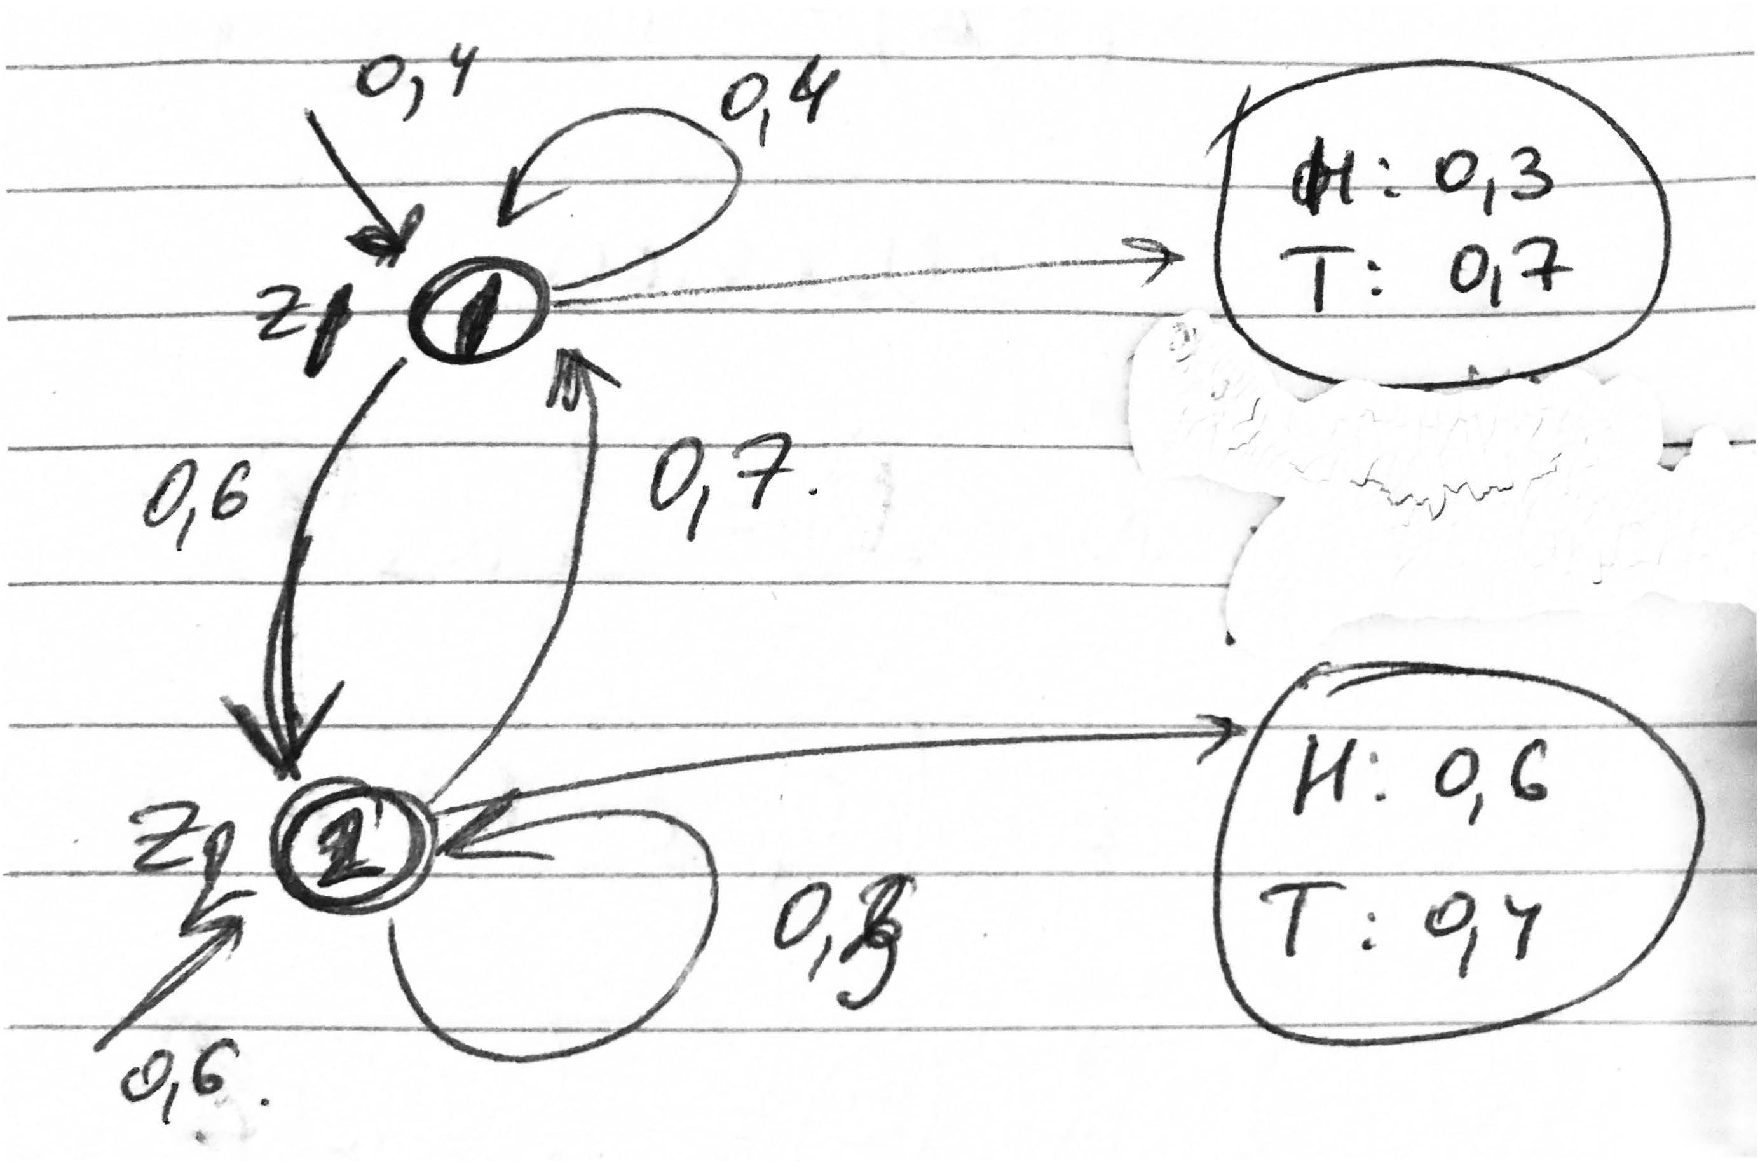
\includegraphics[width = 10cm]{figures/diagram.pdf}}
		\caption{Transition diagram of latent variables states with emission probabilities}
		\label{fig:diagram}
	\end{figure}
	
	\subsection*{Exercise 2.1}
	
	We observe sequence $ O=THTH$.
	
	To compute the forward variable $\alpha$ and the backward variable $\beta$ we make use of forward-backward algorithm and unfold a state transition diagram over time into a lattice \ref{fig:lattice}:
	
	\begin{figure}[H]
		\centering{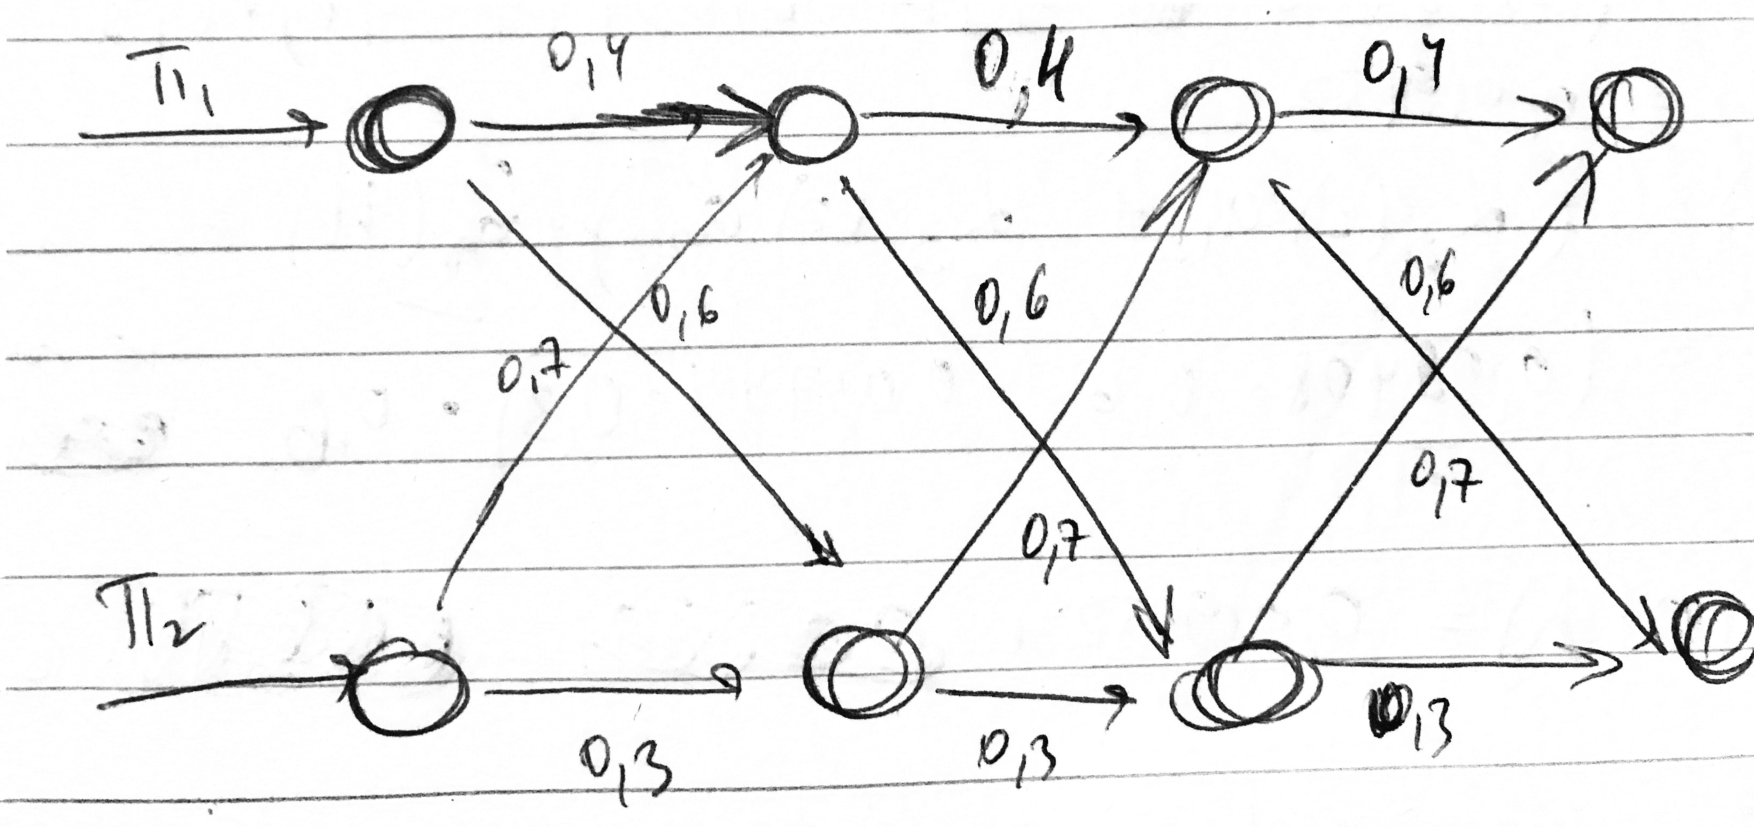
\includegraphics[width = 10cm]{figures/lattice.pdf}}
		\caption{Lattice over time}
		\label{fig:lattice}
	\end{figure}
	
	We use the following formulae for $\alpha$ computation:
	
	$$ \alpha_1(i) = \pi_i \cdot b_i(O_1), \quad \alpha_{t+1} = \left[ \sum_{i=1}^2 \alpha_t(i) \cdot A_{ij} \right] \cdot b_j (O_{t+1})$$
	
	
	\begin{itemize}
	\item $\alpha_1^1(1) = \pi_1 \cdot b_1(T) = 0.4 \cdot 0.7 = 0.28$
	\item $\alpha_1^1(2) = \pi_2 \cdot b_2(T) = 0.6 \cdot 0.4 = 0.24$
	\item $\alpha_2^1(1) = (\alpha_1^1(1) \cdot A_{11} + \alpha_1^1(2) \cdot A_{21}) \cdot b_1(H) = (0.28 \cdot 0.4 + 0.24 \cdot 0.7) \cdot 0.3 = 0.084$
	\item $\alpha_2^1(2) = (\alpha_1^1(1) \cdot A_{12} + \alpha_1^1(2) \cdot A_{22}) \cdot b_2(H) = (0.28 \cdot 0.6 + 0.24 \cdot 0.3) \cdot 0.6 = 0.144$
	\item $\alpha_3^1(1) = (\alpha_2^1(1) \cdot A_{11} + \alpha_2^1(2) \cdot A_{21}) \cdot b_1(T) = (0.084 \cdot 0.4 + 0.144 \cdot 0.7) \cdot 0.7 = 0.09408$
	\item $\alpha_3^1(2) = (\alpha_2^1(1) \cdot A_{12} + \alpha_2^1(2) \cdot A_{22}) \cdot b_2(T) = (0.084 \cdot 0.6 + 0.144 \cdot 0.3) \cdot 0.4 = 0.03744$
	\item $\alpha_4^1(1) = (\alpha_3^1(1) \cdot A_{11} + \alpha_3^1(2) \cdot A_{21}) \cdot b_1(H) = (0.09408 \cdot 0.4 + 0.03744 \cdot 0.7) \cdot 0.3 = 0.019152$	
	\item $\alpha_4^1(2) = (\alpha_3^1(1) \cdot A_{12} + \alpha_3^1(2) \cdot A_{22}) \cdot b_2(H) = (0.09408 \cdot 0.6 + 0.03744 \cdot 0.3) \cdot 0.6 = 0.040608$
	
	\end{itemize}
	
	Similarly we use a recursion relation for $\beta$:
	
	$$ \beta_4(i) = 1, \quad \beta_t(i) = \sum_{j = 1}^2 A_{ij} \cdot b_j(O_{t + 1}) \cdot \beta_{t + 1}(j)$$
	
	\begin{itemize}
		\item $ \beta_4^1(1) = 1 $
		\item $ \beta_4^1(2) = 1 $
		\item $ \beta_3^1(1) = A_{11} \cdot b_1(H) \cdot \beta_4^1(1) +  A_{12} \cdot b_2(H) \cdot \beta_4^1(2) = 0.4 \cdot 0.3 \cdot 1 + 0.6 \cdot 0.6 \cdot 1 = 0.48$
		\item $ \beta_3^1(2) = A_{21} \cdot b_1(H) \cdot \beta_4^1(1) +  A_{22} \cdot b_2(H) \cdot \beta_4^1(2) = 0.7 \cdot 0.3 \cdot 1 + 0.3 \cdot 0.6 \cdot 1 = 0.39$
		\item $ \beta_2^1(1) = A_{11} \cdot b_1(T) \cdot \beta_3^1(1) +  A_{12} \cdot b_2(T) \cdot \beta_3^1(2) = 0.4 \cdot 0.7 \cdot 0.48 + 0.6 \cdot 0.4 \cdot 0.39 = 0.228$
		\item $ \beta_2^1(2) = A_{21} \cdot b_1(T) \cdot \beta_3^1(1) +  A_{22} \cdot b_2(T) \cdot \beta_3^1(2) = 0.7 \cdot 0.7 \cdot 0.48 + 0.3 \cdot 0.4 \cdot 0.39 = 0.282$
		\item $ \beta_1^1(1) = A_{11} \cdot b_1(H) \cdot \beta_2^1(1) +  A_{12} \cdot b_2(H) \cdot \beta_2^1(2) = 0.4 \cdot 0.3 \cdot 0.228 + 0.6 \cdot 0.6 \cdot 0.282 = 0.12888$
		\item $ \beta_1^1(2) = A_{21} \cdot b_1(H) \cdot \beta_2^1(1) +  A_{22} \cdot b_2(H) \cdot \beta_2^1(2) = 0.7 \cdot 0.3 \cdot 0.228 + 0.3 \cdot 0.6 \cdot 0.282 = 0.09864$
	\end{itemize}
	
	\subsection*{Exercise 2.2}
	
	If we look at our hidden Markov model unfolded over time as at the Bayesian network (Figure \ref{fig:network}), we can find $P(O | M) $ with the help of marginalisation.
	
	\begin{figure}[H]
		\centering{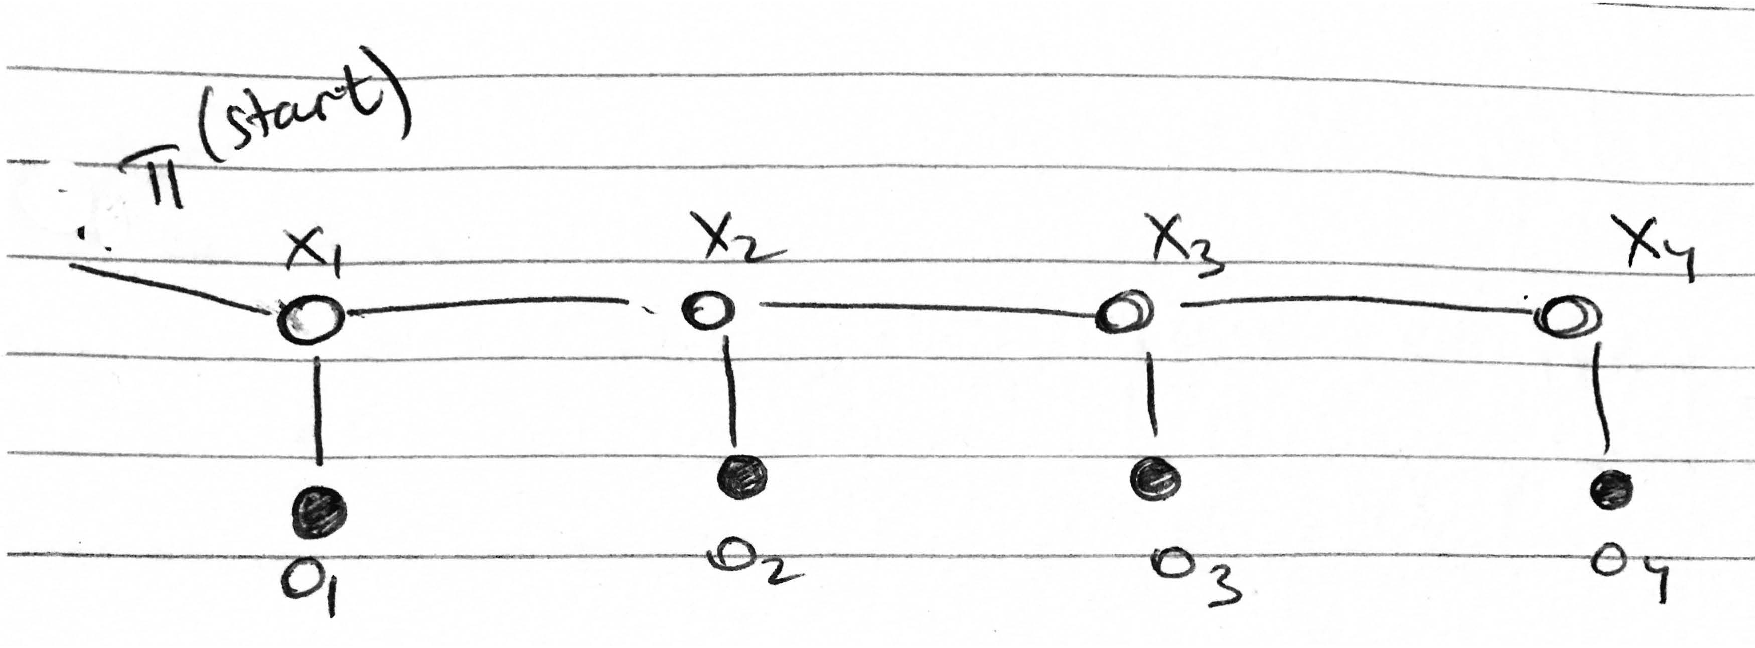
\includegraphics[width = 10cm]{figures/network.pdf}}
		\caption{Network unfolded in time}
		\label{fig:network}
	\end{figure}
	
	$$ p(O) = \sum_{x_1, x_2, x_3, x_4} p(x_1) p(o_1 | x_1) p(x_2 | x_1) p(o_2 |x_2) p(x_3 |x_2) p(o_3|x_3) p(x_4 |x_3) p(o_4 | x_4) $$
	
	We perform several sum-product reorderings in order to simplify the calculations:
	
	$$ p(x_2) = \phi_1(x_2) = \sum_{x_1} p(x_1) p(o_1 |x_1) p(x_2 | x_1) $$
	
	$$ p(O) = \sum_{x_2, x_3, x_4}p(x_2) p(o_2 |x_2) p(x_3 |x_2) p(o_3|x_3) p(x_4 |x_3) p(o_4 | x_4) $$
	
	$$ p(x_3) = \phi_2(x_3) = \sum_{x_2} p(x_2) p(o_2 |x_2) p(x_3 | x_2) $$
	
	$$ p(O) = \sum_{x_3, x_4} p(x_3) p(o_3|x_3) p(x_4 |x_3) p(o_4 | x_4) $$
	
	$$ p(x_4) = \phi_3(x_4) = \sum_{x_3} p(x_3) p(o_3 |x_3) p(x_4 | x_3) $$
	
	$$ p(O) = \sum_{x_4} p(x_4) p(o_4 | x_4) =  \sum_{x_4} p(o_4, x_4) = \sum_{j} \alpha_4(j)$$ 
	
	$$ p(O^1) = \alpha_4^1(1) + \alpha_4^1(2) = 0.019152 + 0.040608 = 0.05976 $$
	
	
	\subsection*{Exercise 2.3}
	
	In this exercise we are applying one step of the batch approach of EM algorithm. To do so, we need to obtain $\alpha$ and $\beta$ for both observed sequences $O^1 = THTH$ and $O^2 = THHT$, then compute responsibilities $\gamma_t(i)$ and conditional probabilities $\xi_t(i, j)$ (E-step of the algorithm). After that, we update the model parameters (M-step of the algorithm).
	
	We have already computed $\alpha$ and $\beta$ for the first sequence in \textbf{Exercise 2.1}. 
	Now we can compute the responsibilities	$\gamma_t(i)$ for the first sequence:
		
	$$  \gamma_t(i) = \frac{\alpha_t(i) \cdot \beta_t(i)}{\sum_{j = 1}^2 \alpha_t(j) \cdot \beta_t(j)} = \frac{\alpha_t(i) \cdot \beta_t(i)}{p(O)} $$
	\begin{itemize}
		\item $\gamma_1^1(1) = \frac{\alpha_1^1(1) \cdot \beta_1^1(1)}{p(O^1)} =  \frac{0.28 \cdot 0.12888}{0.05976} \approx 0.6039$
		\item $\gamma_1^1(2) = \frac{\alpha_1^1(2) \cdot \beta_1^1(2)}{p(O^1)} =  \frac{0.24 \cdot 0.09864}{0.05976} \approx 0.3961$
		\item $\gamma_2^1(1) = \frac{\alpha_2^1(1) \cdot \beta_2^1(1)}{p(O^1)} =  \frac{0.084 \cdot 0.228}{0.05976} \approx 0.3205$
		\item $\gamma_2^1(2) = \frac{\alpha_2^1(2) \cdot \beta_2^1(2)}{p(O^1)} =  \frac{0.144 \cdot 0.282}{0.05976} \approx 0.6795$
		\item $\gamma_3^1(1) = \frac{\alpha_3^1(1) \cdot \beta_3^1(1)}{p(O^1)} =  \frac{0.09408 \cdot 0.48}{0.05976} \approx 0.7556$
		\item $\gamma_3^1(2) = \frac{\alpha_3^1(2) \cdot \beta_3^1(2)}{p(O^1)} =  \frac{0.03744 \cdot 0.39}{0.05976} \approx 0.2444$
		\item $\gamma_4^1(1) = \frac{\alpha_4^1(1) \cdot \beta_4^1(1)}{p(O^1)} =  \frac{0.019152 \cdot 1}{0.05976} \approx 0.3246$
		\item $\gamma_4^1(2) = \frac{\alpha_4^1(2) \cdot \beta_4^1(2)}{p(O^1)} =  \frac{0.040608 \cdot 1}{0.05976} \approx 0.6795$
	\end{itemize}
	
	
	After that we are ready to estimate conditional probabilities $\xi_t(i, j)$:
	
	$$ \xi_t(i, j) = \frac{\alpha_t(i) \cdot A_{ij} \cdot b_j(O_{t+1}) \beta_{t+1}(j)}{\sum_{k = 1}^2 \sum_{l = 1}^2\alpha_t(k) \cdot A_{kl} \cdot b_l(O_{t+1}) \beta_{t+1}(l)} = \frac{\alpha_t(i) \cdot A_{ij} \cdot b_j(O_{t+1}) \beta_{t+1}(j)}{p(O)} $$
	
	\begin{itemize}
		\item $ \xi_1^1(1, 1) = \frac{\alpha_1^1(1) \cdot A_{11} \cdot b_1(H) \beta_{2}^1(1)}{p(O^1)} =  \frac{0.28 \cdot 0.4 \cdot 0.3 \cdot 0.228}{0.05976} \approx 0.1282 $
		\item $ \xi_1^1(1, 2) = \frac{\alpha_1^1(1) \cdot A_{12} \cdot b_2(H) \beta_{2}^1(2)}{p(O^1)} =  \frac{0.28 \cdot 0.6 \cdot 0.6 \cdot 0.282}{0.05976} \approx 0.4757 $
		\item $ \xi_1^1(2, 1) = \frac{\alpha_1^1(2) \cdot A_{21} \cdot b_1(H) \beta_{2}^1(1)}{p(O^1)} =  \frac{0.24 \cdot 0.7 \cdot 0.3 \cdot 0.228}{0.05976} \approx 0.1923 $
		\item $ \xi_1^1(2, 2) = \frac{\alpha_1^1(2) \cdot A_{22} \cdot b_2(H) \beta_{2}^1(2)}{p(O^1)} =  \frac{0.24 \cdot 0.3 \cdot 0.6 \cdot 0.282}{0.05976}\approx 0.2038 $
		\item $ \xi_2^1(1, 1) = \frac{\alpha_2^1(1) \cdot A_{11} \cdot b_1(T) \beta_{3}^1(1)}{p(O^1)}=  \frac{0.084 \cdot 0.4 \cdot 0.7 \cdot 0.48}{0.05976} \approx 0.1889 $
		\item $ \xi_2^1(1, 2) = \frac{\alpha_2^1(1) \cdot A_{12} \cdot b_2(T) \beta_{3}^1(2)}{p(O^1)} =  \frac{0.084 \cdot 0.6 \cdot 0.4 \cdot 0.39}{0.05976} \approx 0.1316 $
		\item $ \xi_2^1(2, 1) = \frac{\alpha_2^1(2) \cdot A_{21} \cdot b_1(T) \beta_{3}^1(1)}{p(O^1)} =  \frac{0.144 \cdot 0.7 \cdot 0.7 \cdot 0.48}{0.05976} \approx 0.5667 $
		\item $ \xi_2^1(2, 2) = \frac{\alpha_2^1(2) \cdot A_{22} \cdot b_2(T) \beta_{3}^1(2)}{p(O^1)}=  \frac{0.144 \cdot 0.3 \cdot 0.4 \cdot 0.39}{0.05976} \approx 0.1128 $
		\item $ \xi_3^1(1, 1) = \frac{\alpha_3^1(1) \cdot A_{11} \cdot b_1(H) \beta_{4}^1(1)}{p(O^1)} =  \frac{0.09408 \cdot 0.4 \cdot 0.3 \cdot 1}{0.05976} \approx 0.1889 $
		\item $ \xi_3^1(1, 2) = \frac{\alpha_3^1(1) \cdot A_{12} \cdot b_2(H) \beta_{4}^1(2)}{p(O^1)} =  \frac{0.09408 \cdot 0.6 \cdot 0.6 \cdot 1}{0.05976} \approx 0.5667 $
		\item $ \xi_3^1(2, 1) = \frac{\alpha_3^1(2) \cdot A_{21} \cdot b_1(H) \beta_{4}^1(1)}{p(O^1)} =  \frac{0.03744 \cdot 0.7 \cdot 0.3 \cdot 1}{0.05976} \approx 0.1316 $
		\item $ \xi_3^1(2, 2) = \frac{\alpha_3^1(2) \cdot A_{22} \cdot b_2(H) \beta_{4}^1(2)}{p(O^1)}=  \frac{0.03744 \cdot 0.3 \cdot 0.6 \cdot 1}{0.05976} \approx 0.1128 $
	\end{itemize}
	
	
Similarly, we perform all the computations for observed sequence $O^2 = THHT$.

\begin{itemize}
	\item $\alpha_1^2(1) = 0.28$
	\item $\alpha_1^2(2) = 0.24$
	\item $\alpha_2^2(1) = 0.084$
	\item $\alpha_2^2(2) = 0.144$
	\item $\alpha_3^2(1) = (\alpha_2^2(1) \cdot A_{11} + \alpha_2^2(2) \cdot A_{21}) \cdot b_1(H) = (0.084 \cdot 0.4 + 0.144 \cdot 0.7) \cdot 0.3 = 0.04032$
	\item $\alpha_3^2(2) = (\alpha_2^2(1) \cdot A_{12} + \alpha_2^2(2) \cdot A_{22}) \cdot b_2(H) = (0.084 \cdot 0.6 + 0.144 \cdot 0.3) \cdot 0.6 = 0.05616$
	\item $\alpha_4^2(1) = (\alpha_3^2(1) \cdot A_{11} + \alpha_3^2(2) \cdot A_{21}) \cdot b_1(T) = (0.04032 \cdot 0.4 + 0.05616 \cdot 0.7) \cdot 0.7 = 0.038808$	
	\item $\alpha_4^2(2) = (\alpha_3^2(1) \cdot A_{12} + \alpha_3^2(2) \cdot A_{22}) \cdot b_2(T) = (0.04032 \cdot 0.6 + 0.05616 \cdot 0.3) \cdot 0.4 = 0.016416$
	
\end{itemize}

	$$ p(O^2) = \sum_{j} \alpha_4^2(j) = \alpha_4^2(1) + \alpha_4^2(2) = 0.038808 + 0.016416 = 0.055224 $$ 
	
	\begin{itemize}
		\item $ \beta_4^2(1) = 1 $
		\item $ \beta_4^2(2) = 1 $
		\item $ \beta_3^2(1) = A_{11} \cdot b_1(T) \cdot \beta_4^2(1) +  A_{12} \cdot b_2(T) \cdot \beta_4^2(2) = 0.4 \cdot 0.7 \cdot 1 + 0.6 \cdot 0.4 \cdot 1 = 0.52$
		\item $ \beta_3^2(2) = A_{21} \cdot b_1(T) \cdot \beta_4^2(1) +  A_{22} \cdot b_2(T) \cdot \beta_4^2(2) = 0.7 \cdot 0.7 \cdot 1 + 0.3 \cdot 0.4 \cdot 1 = 0.61$
		\item $ \beta_2^2(1) = A_{11} \cdot b_1(H) \cdot \beta_3^2(1) +  A_{12} \cdot b_2(H) \cdot \beta_3^2(2) = 0.4 \cdot 0.3 \cdot 0.52 + 0.6 \cdot 0.6 \cdot 0.61 = 0.282$
		\item $ \beta_2^2(2) = A_{21} \cdot b_1(H) \cdot \beta_3^2(1) +  A_{22} \cdot b_2(H) \cdot \beta_3^2(2) = 0.7 \cdot 0.3 \cdot 0.52 + 0.3 \cdot 0.6 \cdot 0.61 = 0.219$
		\item $ \beta_1^2(1) = A_{11} \cdot b_1(H) \cdot \beta_2^2(1) +  A_{12} \cdot b_2(H) \cdot \beta_2^2(2) = 0.4 \cdot 0.3 \cdot 0.282 + 0.6 \cdot 0.6 \cdot 0.219 = 0.11268$
		\item $ \beta_1^2(2) = A_{21} \cdot b_1(H) \cdot \beta_2^2(1) +  A_{22} \cdot b_2(H) \cdot \beta_2^2(2) = 0.7 \cdot 0.3 \cdot 0.282 + 0.3 \cdot 0.6 \cdot 0.219 = 0.09864$
	\end{itemize}
	
	\begin{itemize}
		\item $\gamma_1^2(1) = \frac{\alpha_1^1(1) \cdot \beta_1^1(1)}{p(O^1)} =  \frac{0.28 \cdot 0.11268}{0.055224} \approx 0.5713$
		\item $\gamma_1^2(2) = \frac{\alpha_1^1(2) \cdot \beta_1^1(2)}{p(O^1)} =  \frac{0.24 \cdot 0.09864}{0.055224} \approx 0.4287$
		\item $\gamma_2^2(1) = \frac{\alpha_2^1(1) \cdot \beta_2^1(1)}{p(O^1)} =  \frac{0.084 \cdot 0.282}{0.055224} \approx 0.429$
		\item $\gamma_2^2(2) = \frac{\alpha_2^1(2) \cdot \beta_2^1(2)}{p(O^1)} =  \frac{0.144 \cdot 0.219}{0.055224} \approx 0.571$
		\item $\gamma_3^2(1) = \frac{\alpha_3^1(1) \cdot \beta_3^1(1)}{p(O^1)} =  \frac{0.04032 \cdot 0.52}{0.055224} \approx 0.3797$
		\item $\gamma_3^2(2) = \frac{\alpha_3^1(2) \cdot \beta_3^1(2)}{p(O^1)} =  \frac{0.05616 \cdot 0.61}{0.055224} \approx 0.6203$
		\item $\gamma_4^2(1) = \frac{\alpha_4^1(1) \cdot \beta_4^1(1)}{p(O^1)} =  \frac{0.038808 \cdot 1}{0.055224} \approx 0.7027$
		\item $\gamma_4^2(2) = \frac{\alpha_4^1(2) \cdot \beta_4^1(2)}{p(O^1)} =  \frac{0.016416 \cdot 1}{0.055224} \approx 0.2973$
	\end{itemize}
	
	\begin{itemize}
		\item $ \xi_1^2(1, 1) = \frac{\alpha_1^2(1) \cdot A_{11} \cdot b_1(H) \beta_{2}^2(1)}{p(O^2)} =  \frac{0.28 \cdot 0.4 \cdot 0.3 \cdot 0.282}{0.055224} \approx 0.1716 $
		\item $ \xi_1^2(1, 2) = \frac{\alpha_1^2(1) \cdot A_{12} \cdot b_2(H) \beta_{2}^2(2)}{p(O^2)} =  \frac{0.28 \cdot 0.6 \cdot 0.6 \cdot 0.219}{0.055224} \approx 0.2997 $
		\item $ \xi_1^2(2, 1) = \frac{\alpha_1^2(2) \cdot A_{21} \cdot b_1(H) \beta_{2}^2(1)}{p(O^2)} =  \frac{0.24 \cdot 0.7 \cdot 0.3 \cdot 0.282}{0.055224} \approx 0.2574 $
		\item $ \xi_1^2(2, 2) = \frac{\alpha_1^2(2) \cdot A_{22} \cdot b_2(H) \beta_{2}^2(2)}{p(O^2)} =  \frac{0.24 \cdot 0.3 \cdot 0.6 \cdot 0.219}{0.055224}\approx 0.1713 $
		\item $ \xi_2^2(1, 1) = \frac{\alpha_2^2(1) \cdot A_{11} \cdot b_1(H) \beta_{3}^2(1)}{p(O^2)}=  \frac{0.084 \cdot 0.4 \cdot 0.3 \cdot 0.52}{0.055224} \approx 0.0949 $
		\item $ \xi_2^2(1, 2) = \frac{\alpha_2^2(1) \cdot A_{12} \cdot b_2(H) \beta_{3}^2(2)}{p(O^2)} =  \frac{0.084 \cdot 0.6 \cdot 0.6 \cdot 0.61}{0.055224} \approx 0.3341 $
		\item $ \xi_2^2(2, 1) = \frac{\alpha_2^2(2) \cdot A_{21} \cdot b_1(H) \beta_{3}^2(1)}{p(O^2)} =  \frac{0.144 \cdot 0.7 \cdot 0.3 \cdot 0.52}{0.055224} \approx 0.2847 $
		\item $ \xi_2^2(2, 2) = \frac{\alpha_2^2(2) \cdot A_{22} \cdot b_2(H) \beta_{3}^2(2)}{p(O^2)}=  \frac{0.144 \cdot 0.3 \cdot 0.6 \cdot 0.61}{0.055224} \approx 0.2863 $
		\item $ \xi_3^2(1, 1) = \frac{\alpha_3^2(1) \cdot A_{11} \cdot b_1(T) \beta_{4}^2(1)}{p(O^2)} =  \frac{0.04032 \cdot 0.4 \cdot 0.7 \cdot 1}{0.055224} \approx 0.2044 $
		\item $ \xi_3^2(1, 2) = \frac{\alpha_3^2(1) \cdot A_{12} \cdot b_2(T) \beta_{4}^2(2)}{p(O^2)} =  \frac{0.04032 \cdot 0.6 \cdot 0.4 \cdot 1}{0.055224} \approx 0.1753 $
		\item $ \xi_3^2(2, 1) = \frac{\alpha_3^2(2) \cdot A_{21} \cdot b_1(T) \beta_{4}^2(1)}{p(O^2)} =  \frac{0.05616 \cdot 0.7 \cdot 0.7 \cdot 1}{0.055224} \approx 0.4983 $
		\item $ \xi_3^2(2, 2) = \frac{\alpha_3^2(2) \cdot A_{22} \cdot b_2(T) \beta_{4}^2(2)}{p(O^2)}=  \frac{0.05616 \cdot 0.3 \cdot 0.4 \cdot 1}{0.055224} \approx 0.122 $
	\end{itemize}
	
	
	
	After that we have everything to perform M-step of the EM-algorithm.
	
	First, we reestimate the initial probabilities:
	
	$$\widehat{\pi_i} = \frac{\sum_{k=1}^K \gamma_1^k(i)}{K} $$
	
	\begin{itemize}
		\item $ \widehat{\pi_1} = \frac{ \gamma_1^1(1) +  \gamma_1^2(1)}{2} = \frac{ 0.6039 + 0.5713}{2} = 0.5876$
		\item $ \widehat{\pi_2}= \frac{ \gamma_1^1(2) +  \gamma_1^2(2)}{2} = \frac{ 0.3961 + 0.4287}{2} = 0.4124$
	\end{itemize}	
	
	$$ \widehat{\pi} = (0.5876, 0.4124) $$
	
	Furthemore, we recompute the transition probabilities:
	
	$$ \widehat{A_{ij}} = \frac{\sum_{k=1}^K \sum_{t = 1}^{T_k - 1} \xi_t^k(i, j) }{\sum_{k=1}^K \sum_{t = 1}^{T_k - 1} \gamma_t^k(i) } $$
	
	\begin{itemize}
		\item $ \widehat{A_{11}} = \frac{\xi_1^1(1, 1) + \xi_2^1(1, 1) + \xi_3^1(1, 1) + \xi_1^2(1, 1) + \xi_2^2(1, 1)+ \xi_3^2(1, 1) }{ \gamma_1^1(1) + \gamma_2^1(1) + \gamma_3^1(1) + \gamma_1^2(1) + \gamma_2^2(1) + \gamma_3^2(1)} \approx 0.3192 $ 
		\item $ \widehat{A_{12}} = \frac{\xi_1^1(1, 2) + \xi_2^1(1, 2) + \xi_3^1(1, 2) + \xi_1^2(1, 2) + \xi_2^2(1, 2)+ \xi_3^2(1, 2) }{ \gamma_1^1(1) + \gamma_2^1(1) + \gamma_3^1(1) + \gamma_1^2(1) + \gamma_2^2(1) + \gamma_3^2(1)} \approx 0.6808 $ 
		\item $ \widehat{A_{21}} = \frac{\xi_1^1(2, 1) + \xi_2^1(2, 1) + \xi_3^1(2, 1) + \xi_1^2(2, 1) + \xi_2^2(2, 1)+ \xi_3^2(2, 1) }{ \gamma_1^1(2) + \gamma_2^1(2) + \gamma_3^1(2) + \gamma_1^2(2) + \gamma_2^2(2) + \gamma_3^2(2)} \approx 0.6568 $ 
		\item $ \widehat{A_{22}} = \frac{\xi_1^1(2, 2) + \xi_2^1(2, 2) + \xi_3^1(2, 2) + \xi_1^2(2, 2) + \xi_2^2(2, 2)+ \xi_3^2(2, 2) }{ \gamma_1^1(2) + \gamma_2^1(2) + \gamma_3^1(2) + \gamma_1^2(2) + \gamma_2^2(2) + \gamma_3^2(2)} \approx 0.3432 $ 
	\end{itemize}
	
	
	$$ \widehat{A} = \left(\begin{smallmatrix} 0.3192 & 0.6808  \\ \\ 0.6568 & 0.3432  \end{smallmatrix} \right)$$
	
	Finally, we recalculate the emission probabilities. Let's summarize what responsibilities we obtained so far (the third column stands for the observed variable at this point):
	$$ \gamma^1(z_1, z_2) = \left(\begin{smallmatrix} 0.6039 & 0.3961 & (T) \\ \\ 0.3205 & 0.6795 & (H) \\ \\ 0.7556 & 0.2444 & (T) \\ \\ 0.3245 & 0.6795 & (H) \end{smallmatrix} \right)  $$
	
	$$ \gamma^2(z_1, z_2) = \left(\begin{smallmatrix} 0.5713 & 0.4287 & (T) \\ \\ 0.429 & 0.571 & (H) \\ \\ 0.3797 & 0.6203 & (H) \\ \\ 0.7027 & 0.2973 & (T) \end{smallmatrix} \right)  $$
	
	$$ b_j(v_m) = \frac{\sum_{k=1}^K \sum_{t = 1}^{T_k}  \gamma_t^k(j) 1(O_t^k = v_m) }{ \sum_{k=1}^K \sum_{t = 1}^{T_k}  \gamma_t^k(i) } $$
	
	
	\begin{itemize}
		\item We choose all the responsibilities for $z_1$ when the observed variable is $H$: \\
		$ \widehat{b_1}(H) = \frac{\gamma_2^1(1) + \gamma_4^1(1) + \gamma_2^2(1) + \gamma_3^2(1)}{ \gamma_1^1(1) + \gamma_2^1(1) + \gamma_3^1(1)  + \gamma_4^1(1) + \gamma_1^2(1) + \gamma_2^2(1) + \gamma_3^2(1) + \gamma_4^2(1) } \approx 0.3557$
		
		\item We choose all the responsibilities for $z_1$ when the observed variable is $T$: \\
		$ \widehat{b_1}(T) = \frac{\gamma_1^1(1) + \gamma_3^1(1) + \gamma_1^2(1) + \gamma_4^2(1)}{ \gamma_1^1(1) + \gamma_2^1(1) + \gamma_3^1(1)  + \gamma_4^1(1) + \gamma_1^2(1) + \gamma_2^2(1) + \gamma_3^2(1) + \gamma_4^2(1) } \approx 0.6443$
		
		\item We choose all the responsibilities for $z_2$ when the observed variable is $H$: \\
		$ \widehat{b_2}(H) = \frac{\gamma_2^1(2) + \gamma_4^1(2) + \gamma_2^2(2) + \gamma_3^2(2)}{ \gamma_1^1(2) + \gamma_2^1(2) + \gamma_3^1(2)  + \gamma_4^1(2) + \gamma_1^2(2) + \gamma_2^2(2) + \gamma_3^2(2) + \gamma_4^2(2) } \approx 0.6541$
		
		\item We choose all the responsibilities for $z_2$ when the observed variable is $T$: \\
		$ \widehat{b_2}(T) = \frac{\gamma_1^1(2) + \gamma_3^1(2) + \gamma_1^2(2) + \gamma_4^2(2)}{ \gamma_1^1(2) + \gamma_2^1(2) + \gamma_3^1(2)  + \gamma_4^1(2) + \gamma_1^2(2) + \gamma_2^2(2) + \gamma_3^2(2) + \gamma_4^2(2) } \approx 0.3459$
	\end{itemize}
	
	$$ \widehat{b_1} = (0.3557, 0.6443), \quad  \widehat{b_2} = (0.6541, 0.3459)$$
	
	
\end{document}

